For testing our package we selected a not yet published, but very complex dataset, for traumatic \gls{sci}, that is a neurological condition occurring mainly at the thoracic and cervical levels.
The dataset is composed of 62 samples of bulk \textit{RNA-seq}, divided into groups of two different tissues at four different time points, with treatments and controls at each time point.

The \gls{tic} pipeline, as described in figure \ref{fig:ticorserflow}, has been applied for this case study.

\begin{figure}[H]
\centering
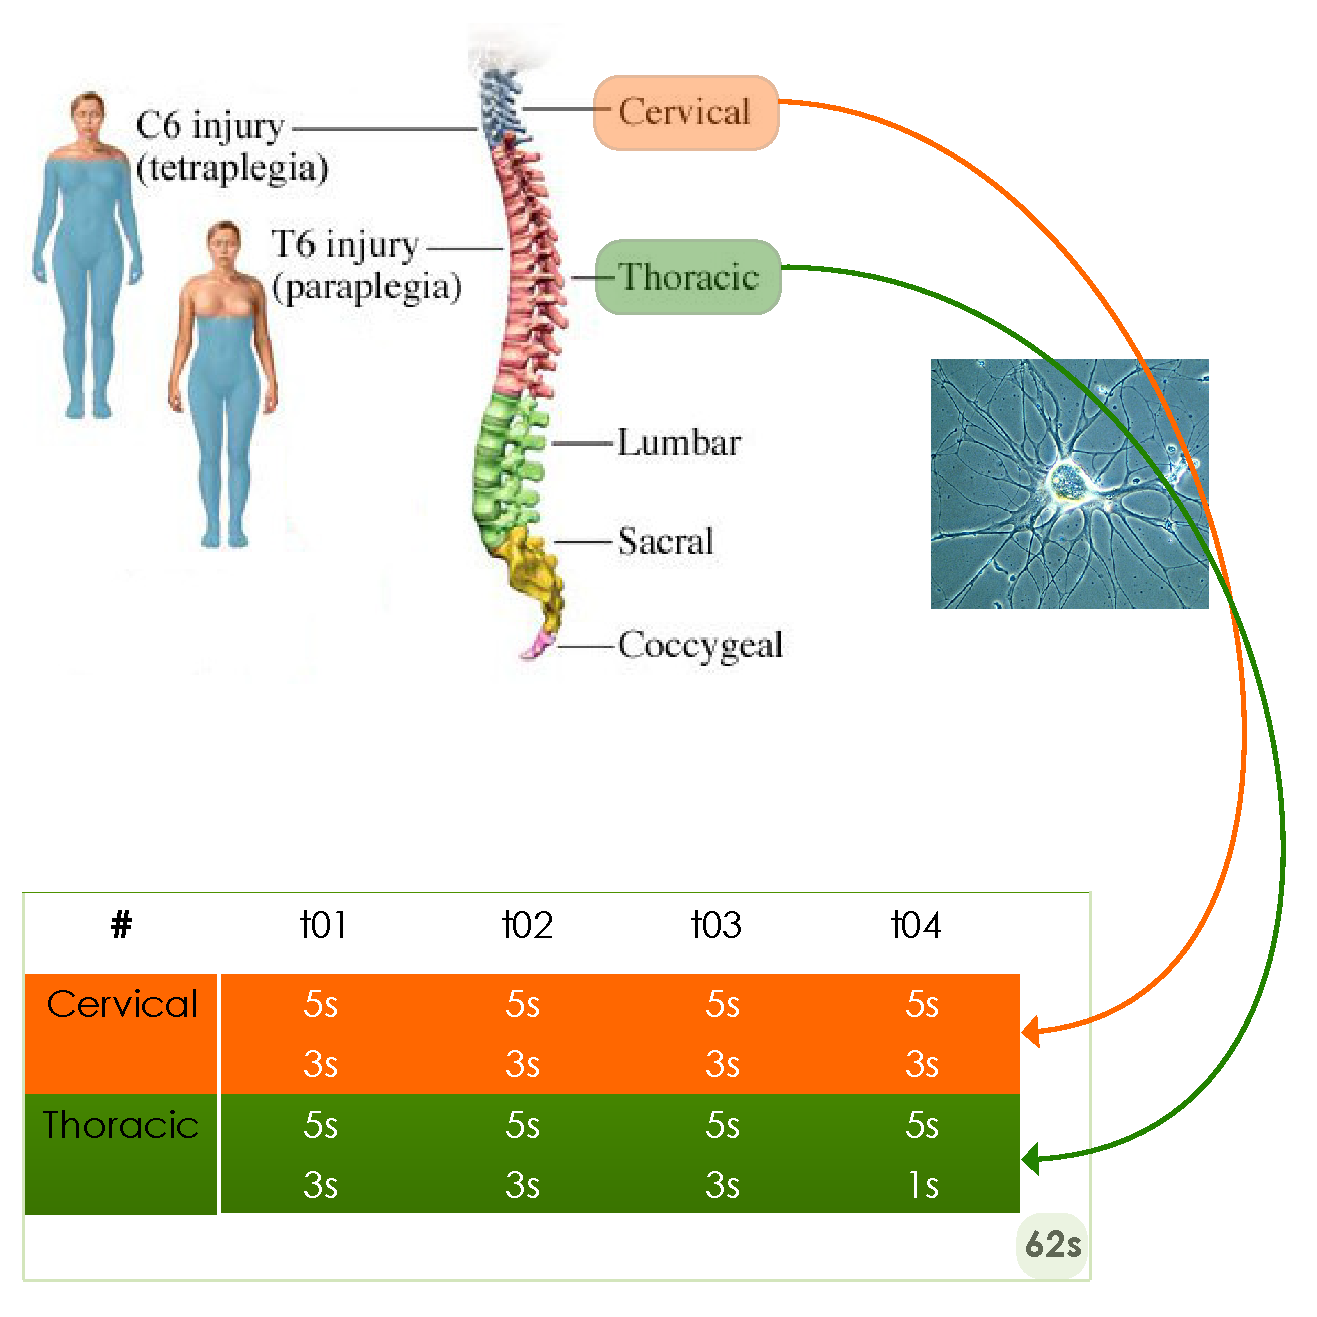
\includegraphics[width=\textwidth, keepaspectratio]{img/ticorser/dataset.pdf}
\caption[ticorser dataset]{An illustrative example of the used dataset. Neurons of Cervical and Thoracic spinal cord injury have been extracted and sequenced at 4 different time points. Inside the table, for each tissue (Cervical/Thoracic) the number of samples for the treatments (upper line) and controls (lower line) are reported at each time point.}
\label{fig:ticorserdataset}

\end{figure}

Because the dataset is not yet accessible, the genes and the samples have been masked during the analysis and no further details will be provided, but we only use it as an illustrative example (figure \ref{fig:ticorserdataset} shows the dataset with most relevant details masked).

\subsubsection{Features quantification}
\gls{tic} gives the possibility to quantify the gene expression by using the \lstinline!featureCounts! method of the \lstinline!rsubread! R/Bioconductor package, by using the \lstinline!countBamFiltesFeatureCounts! method with the path of the \textit{BAM} files and a \gls{gtf}\footnote{https://www.ensembl.org/info/website/upload/gff.html} file within the desired annotation features.

It's really important the choice of the \gls{gtf} file, in terms of version and release, because it affects the further analysis. For this reason, we suggest to always use the latest version of the \gls{gtf} of the genome for the under investigation species \footnote{Two main resources for genome download are https://www.ensembl.org/index.html and https://www.ncbi.nlm.nih.gov/grc}. 

After the gene quantification, the method produces a count matrix with the features (genes) on the rows and the samples on the columns. 
Each cell of the matrix is a discrete value indicating the number of reads quantified for the feature on the row in the column of the sample. 

\subsubsection{The design matrix}
From this point afterwards, \gls{tic} requires a design file illustrating the descriptive characteristics of each sample, in order to speed up the computations and the interactions with the user.
In particular, the design matrix must have the first column specifying the sample names, which has to be equal to the column names in the count matrix.
Table \ref{tab:ticorserdesmat} shows an example of a typical design matrix useful to work with \gls{tic} package.

\begin{table}[H]
\centering
\begin{tabular}{cccc}
\hline\hline
rownames & Times & Conditions & Tissue \\
\hline
s01\_t01\_t1 & 01h & treated1 & tissue1 \\
s02\_t01\_t1 & 01h & treated1 & tissue1 \\
s03\_t01\_t1 & 01h & treated1 & tissue1 \\
s01\_t01\_u1 & 01h & untreated1 & tissue1 \\
s02\_t01\_u1 & 01h & untreated1 & tissue1 \\
s03\_t01\_u1 & 01h & untreated1 & tissue1 \\
s01\_t02\_t1 & 02h & treated1 & tissue1 \\
s02\_t02\_t1 & 02h & treated1 & tissue1 \\
s03\_t02\_t1 & 02h & treated1 & tissue1 \\
s01\_t02\_u1 & 02h & untreated1 & tissue1 \\
s02\_t02\_u1 & 02h & untreated1 & tissue1 \\
s03\_t02\_u1 & 02h & untreated1 & tissue1 \\
s01\_t01\_t2 & 01h & treated2 & tissue2 \\
s02\_t01\_t2 & 01h & treated2 & tissue2 \\
s03\_t01\_t2 & 01h & treated2 & tissue2 \\
s01\_t01\_u2 & 01h & untreated2 & tissue2 \\
s02\_t01\_u2 & 01h & untreated2 & tissue2 \\
s03\_t01\_u2 & 01h & untreated2 & tissue2 \\
s01\_t02\_t2 & 02h & treated2 & tissue2 \\
s02\_t02\_t2 & 02h & treated2 & tissue2 \\
s03\_t02\_t2 & 02h & treated2 & tissue2 \\
s01\_t02\_u2 & 02h & untreated2 & tissue2 \\
s02\_t02\_u2 & 02h & untreated2 & tissue2 \\
s03\_t02\_u2 & 02h & untreated2 & tissue2 \\
\hline
\end{tabular}
\caption[\gls{tic} Design Matrix example]{An example of design matrix required for the right working of \gls{tic} package.
It provides 3 mandatory columns.
The first column describes sample names equal to the column names of the count matrix.
The \textit{Times} column indicates the time points for each samples, while the \textit{Conditions} column specifies the experimental conditions.
Finally, the \textit{Tissue} column (not mandatory) identifies possible multiple tissues.}
\label{tab:ticorserdesmat}
\end{table}

\subsubsection{Filtering \& Normalization}
The count matrix obtained from the quantification step, could reflect the effects of one or more bias due to experimental passages during the library preparation or to different sequencing batches.
In order to account for this, it is a good practice to normalize data, a step which affects the \glspl{deg} detection \cite{Peixoto2015, Soneson2013d, Bullard2010}.
But before normalizing it, because of the presence of several low expressing features, it might also be useful to filter out them, since they are not relevant and may lead to biased results introducing unwanted noise in the analysis. 

Figure \ref{fig:ticorserfiltering} shows the effects of filtering step on row counts (in upper left corner). 
What emerges from this comparison is that low expressed features are in a high amount in raw data, while it is quite un-important the method used for filtering them.

\begin{figure}[H]
\centering
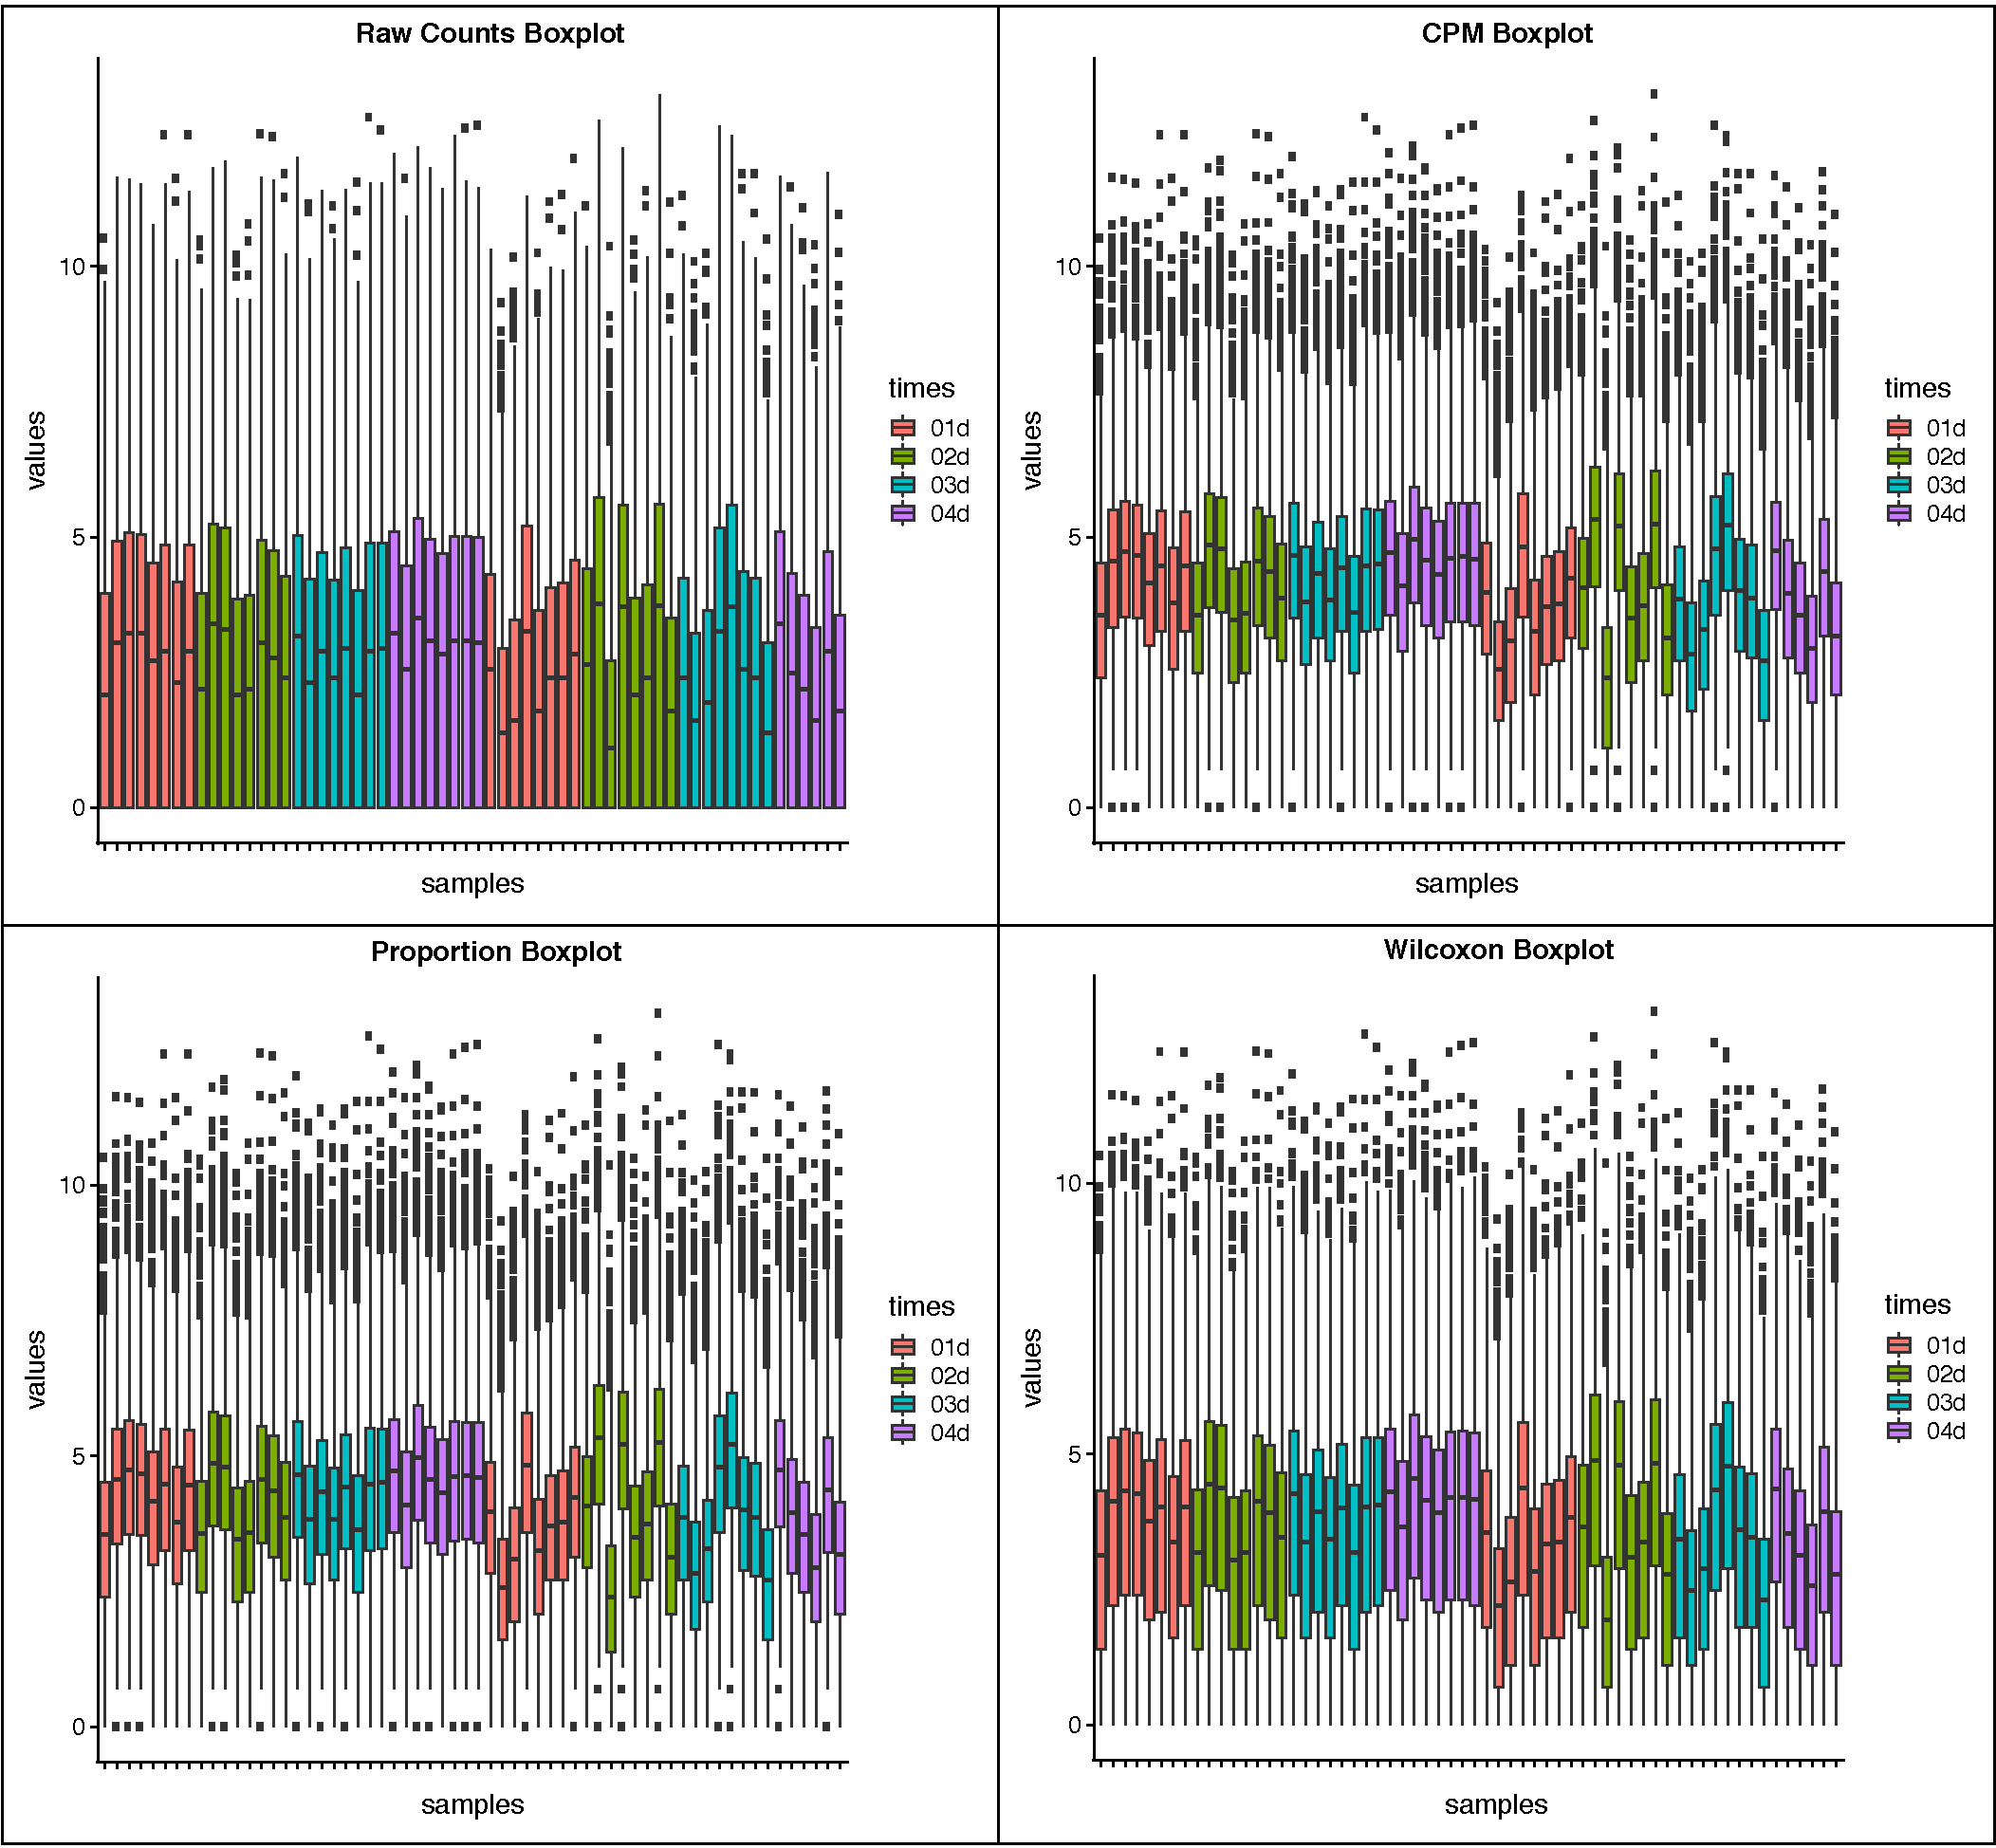
\includegraphics[width=12cm, keepaspectratio]{img/ticorser/filtering/panel1.pdf}
\caption[ticorser filtering methods]{A comparison of how the filtering methods available in \gls{tic} affect the data.
The first panel shows the row counts with low expressed genes, while the other boxes show the filtering effect on the samples.}
\label{fig:ticorserfiltering}

\end{figure}

Moreover, looking at the \textit{Wilcoxon} test, it is more conservative, because it preserves $17039$ features, respect to the \textit{Proportion} test and \gls{cpm}, that preserves, respectively, $14122$ and $14171$ features.
Because of the high numerosity of our samples but low number of replicates are present for each condition, we decided to use the count matrix filtered with \textit{Proportion} test and \lstinline!cpm=1!.

In order to improve the results for the differential expression analysis, it is crucial to correct for between-sample distributional differences in read counts.
To compare the differences of normalized data we decided to use not only the boxplots for the samples, as shown in  figure \ref{fig:ticorsernormalizingbox}, but also the \gls{pca} representation, enabling us to understand which normalization better removes the biases from the samples by clustering the samples of the same group (figure \ref{fig:ticorsernormalizingpca}).

\begin{figure}[H]
\includegraphics[width=12cm,keepaspectratio]{img/ticorser/normalizing/boxplots/all_boxes.pdf}
\caption[ticorser normalizing boxplots]{A comparison of how the normalization methods available in \gls{tic} affect the data.
The first panel shows the row counts with low expressed genes, while the other boxes show the filtering effect on the samples.}
\label{fig:ticorsernormalizingbox}
\centering
\end{figure}

Figure \ref{fig:ticorsernormalizingbox} perfectly shows different effects of each normalization type on count data.  
In fact, we can see that while \textit{Upper quartile} aligns all the samples on the third percentile leaving the medians not aligned, the \textit{Full quantile} applies a stronger effect, which totally aligns the samples, not only on the third percentile but also the medians as such as all the upper distributed outliers.
At the same time, the \textit{TMM} aligns the samples, but in a not so stringent way, well interpreting and leaving the variability of each sample.

\begin{figure}[H]
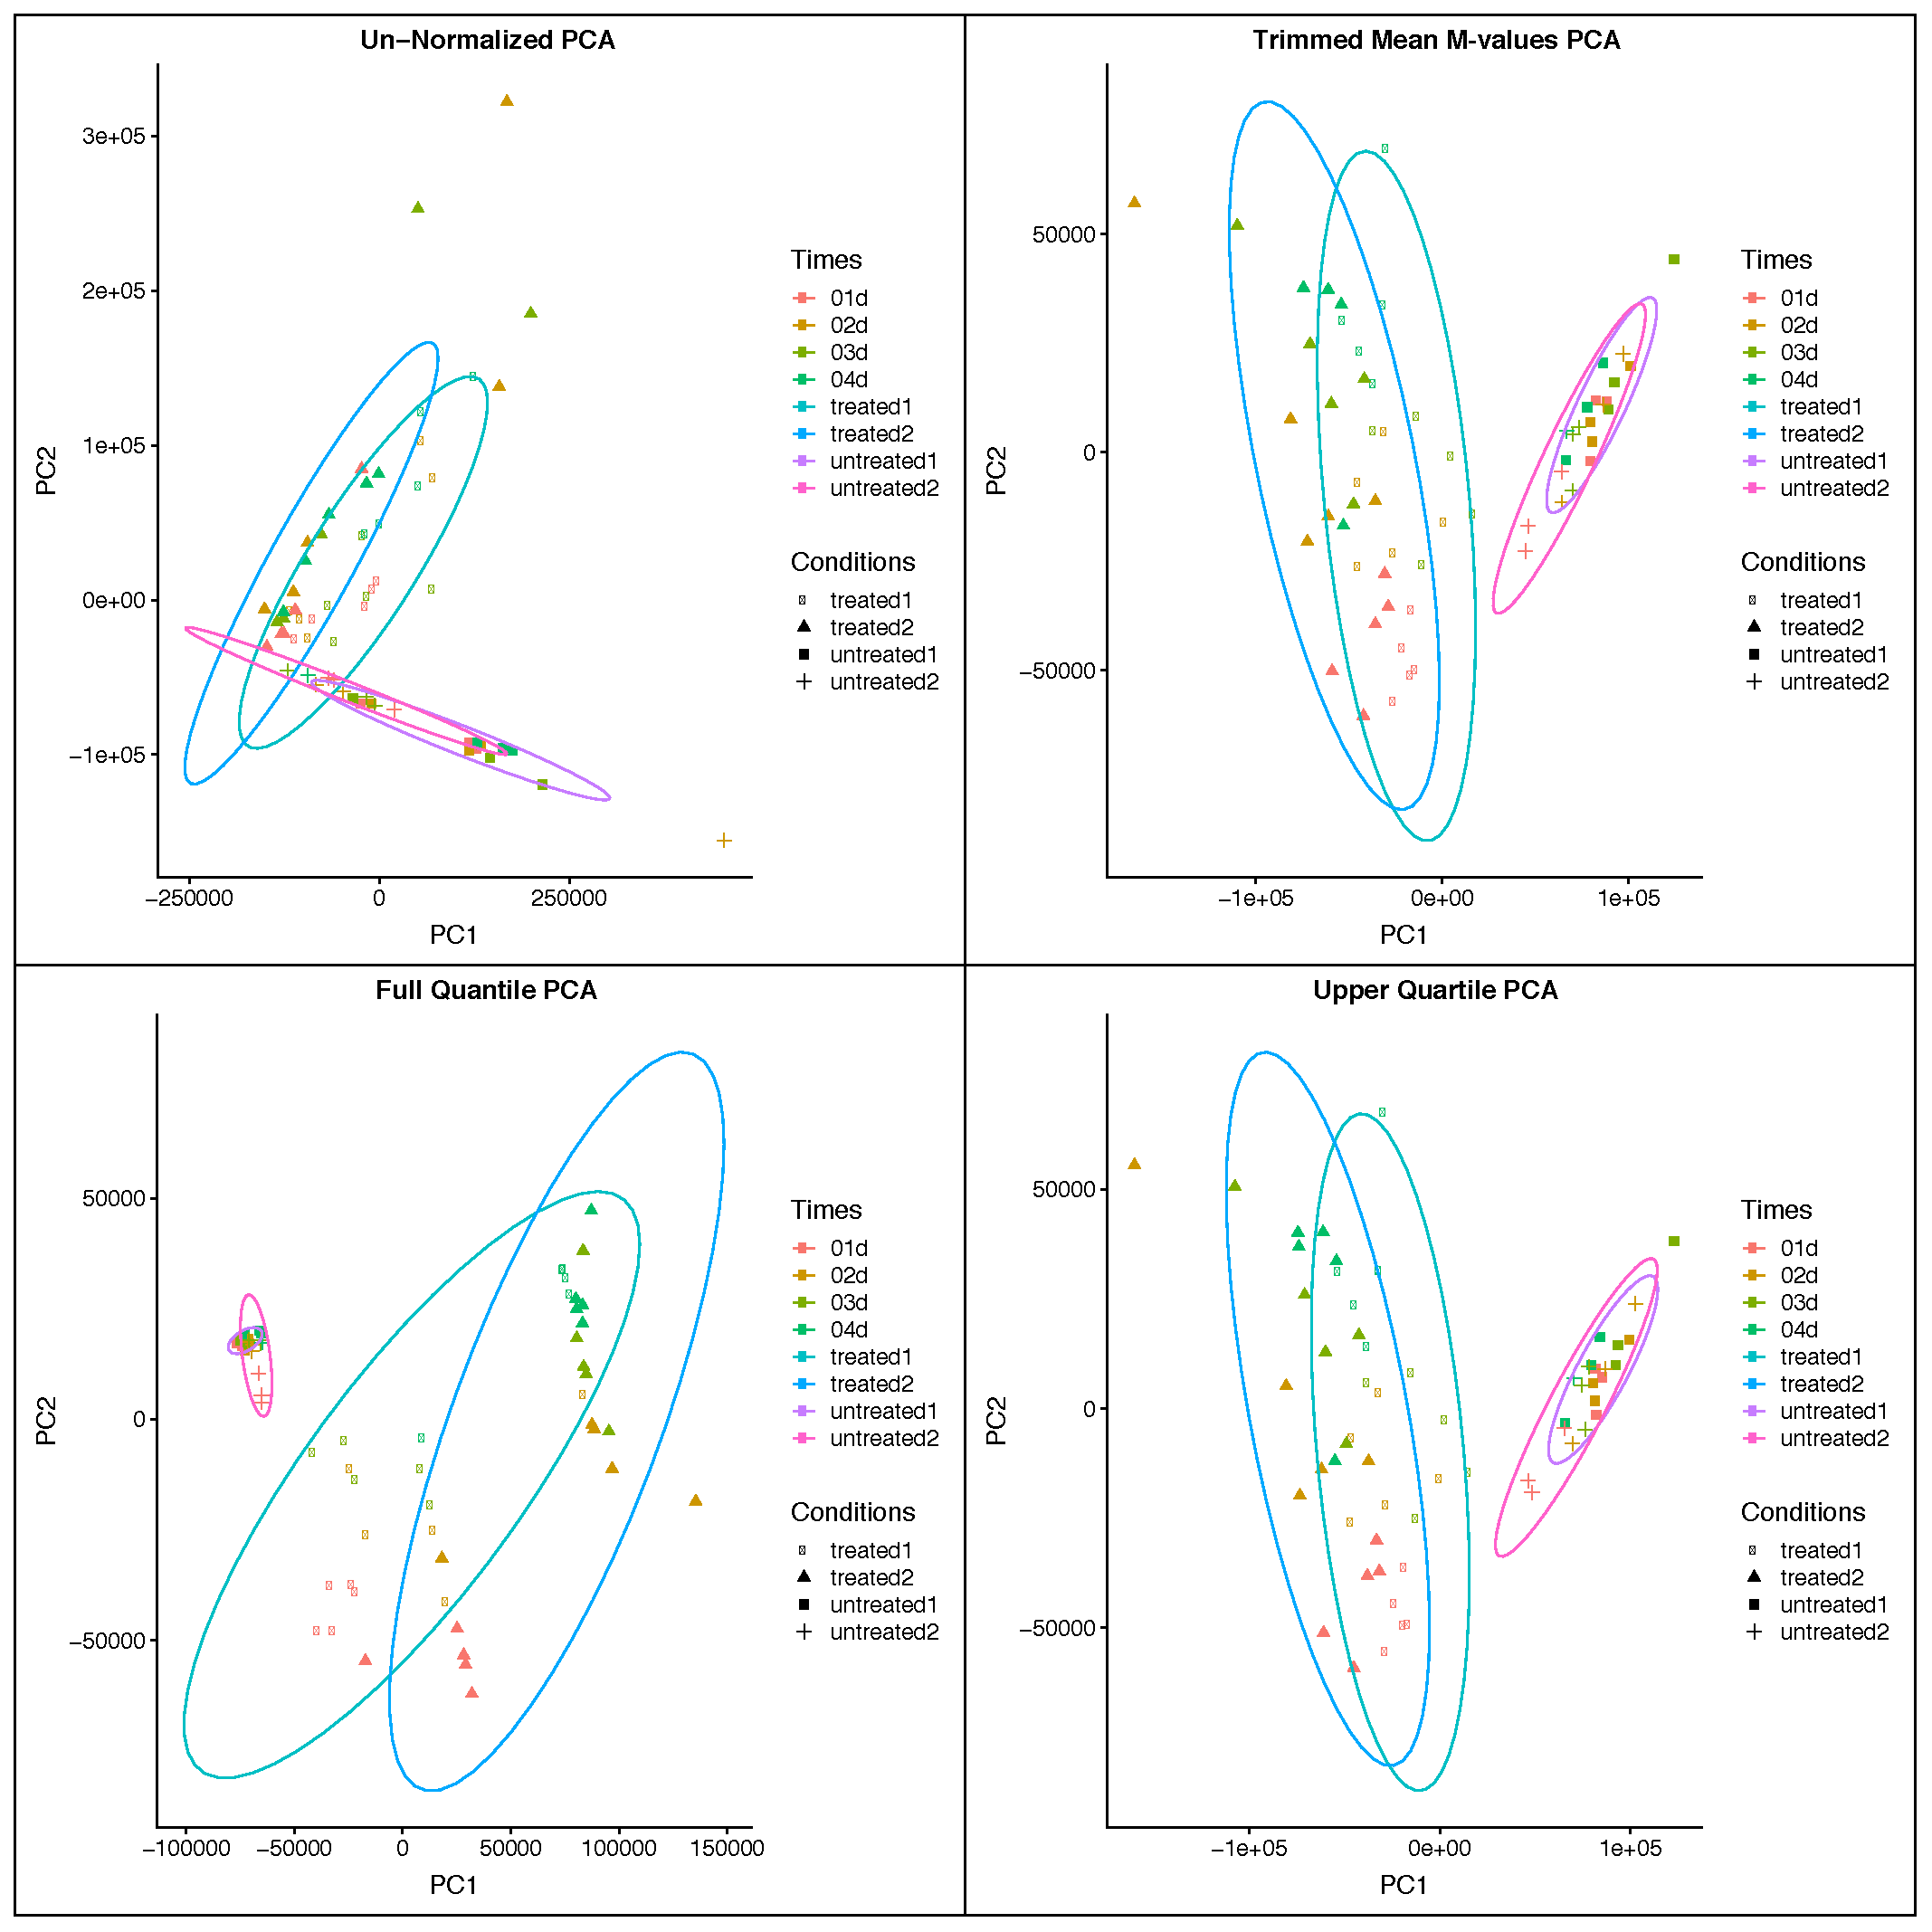
\includegraphics[width=12cm,keepaspectratio]{img/ticorser/normalizing/pca/all_pca.pdf}
\caption[ticorser normalizing \gls{pca}]{A comparison of how the normalizations methods available in \gls{tic} affect the data.
The first panel shows the clustering of row samples, while the other boxes show the normalization effect on the samples.}
\label{fig:ticorsernormalizingpca}
\centering
\end{figure}

As already mentioned a boxplot data inspection could not be enough to determine which normalization method is better working on the data. 
Indeed, when looking at \textit{PCAs} for normalized counts (figure \ref{fig:ticorsernormalizingpca}) the \textit{TMM} and the \textit{Upper quartile} normalizations are able to well discriminate treated and untreated samples, but still preserving some variability inside each group.
While \textit{Full quantile}, even if it is able to help to discriminate the treated and untreated groups, it smashes too much the variability inside untreated samples.

Even if the \textit{TMM} and the \textit{Upper quartile} normalizations seem to affect the data in the same manner, we decided to choose for our further analysis the \textit{Upper quartile} normalized count matrix, because, looking at the \textit{PCA} it seems to better discriminate between the conditions.

\subsubsection{Differential Expression}
Once the data are well normalized, in order to be able to well discriminate between the groups, simply by changing our design matrix with only the interesting samples, we can focus on the differential expression step.
Here we focus only on half of the total dataset, using only the cervical tissue data, checking differences between the treated and untreated samples across experimental time points.

For detecting \glspl{deg} across time points taking into account the conditions we designed \gls{tic} with several methods (see section \ref{sec:ticorsermethods} for further details).
Depending on the biological question under investigation, using the \lstinline!ApplyDeSeq2! function and using the count matrix with the design matrix, the package automatically detects the samples to discriminate for the differential expression.
Moreover, depending on the method selected, it is able to detect different types of genes between the samples.
When selecting \lstinline!DeSeqTime_TC! method, it detects all the genes which change their expression across all time points between two conditions in the \lstinline!Conditions! column of the design matrix, while using \lstinline!DeSeqTime_T!, it recognizes all the genes which have different expression between the conditions across all the time points. 
Furthermore, using \lstinline!DeSeqTime_NoInteraction!, the method is able to detect all those genes demonstrating an oscillating behaviour across the time points in both the conditions.

Additionally, for each of the previously described methods we produce an additional output, applying a \textit{Wald Test} on the \textit{lrt} results, in order to detect all those genes showing differential expression between the two conditions.

For each method we produce a list of two lists, within the results for the \gls{lrt} and for the \textit{LRT\_Wald}. Each of this already divided for all differential expressed gene, only UP genes, only DOWN genes and the results table with all the genes and their statistics.
To identify \glspl{deg} we selected a threshold of $0.05$ on the adjusted p-values, corrected with \gls{fdr} method \cite{Benjamini1995}.

Table \ref{tab:ticorserderesults} illustrates differences in catching \glspl{deg} between the three different methods on the same dataset, highlighting the total number of genes reported, with UP and DOWN regulated. 
It is relevant to see that, when applying the \textit{Wald Test} on the results obtained by \gls{lrt} the \glspl{deg} for this test are much higher in number.

\begin{table}[H]
\centering
\begin{tabular}{r c c c c c c c}
%\cline{2-4}\cline{6-8}
%\cline{2-4}\cline{6-8}
\multicolumn{1}{r}{} & \multicolumn{3}{c}{LRT} && \multicolumn{3}{c}{Wald on LRT} \\
%\cline{2-4}\cline{6-8}
\multicolumn{1}{r}{} & Total & UP & DOWN && Total & UP & DOWN \\
\cline{2-4}\cline{6-8}
TC & 825 & 454 & 371 && 7066 & 3606 & 3460 \\
T & 8812 & 4672 & 4140 && 7066 & 3606 & 3460 \\
No-Int & 9560 & 4893 & 4667 && 9567 & 4900 & 4667 \\
\end{tabular}
\caption[\gls{tic} DE methods results]{This table illustrates differences in catching \glspl{deg} between the three different methods on the same dataset (on the rows), highlighting the total number of genes reported, with UP and DOWN regulated. 
It is relevant to see that, when applying the \textit{Wald Test} on the results obtained by \gls{lrt} the \glspl{deg} for this test are much higher in number.}
\label{tab:ticorserderesults}
\end{table}


It is also possible to inspect the \textit{DE} results by plotting a \textit{Volcano Plot} or an MA plot, as figure \ref{fig:ticorservolcma} shows.

\begin{figure}[H]
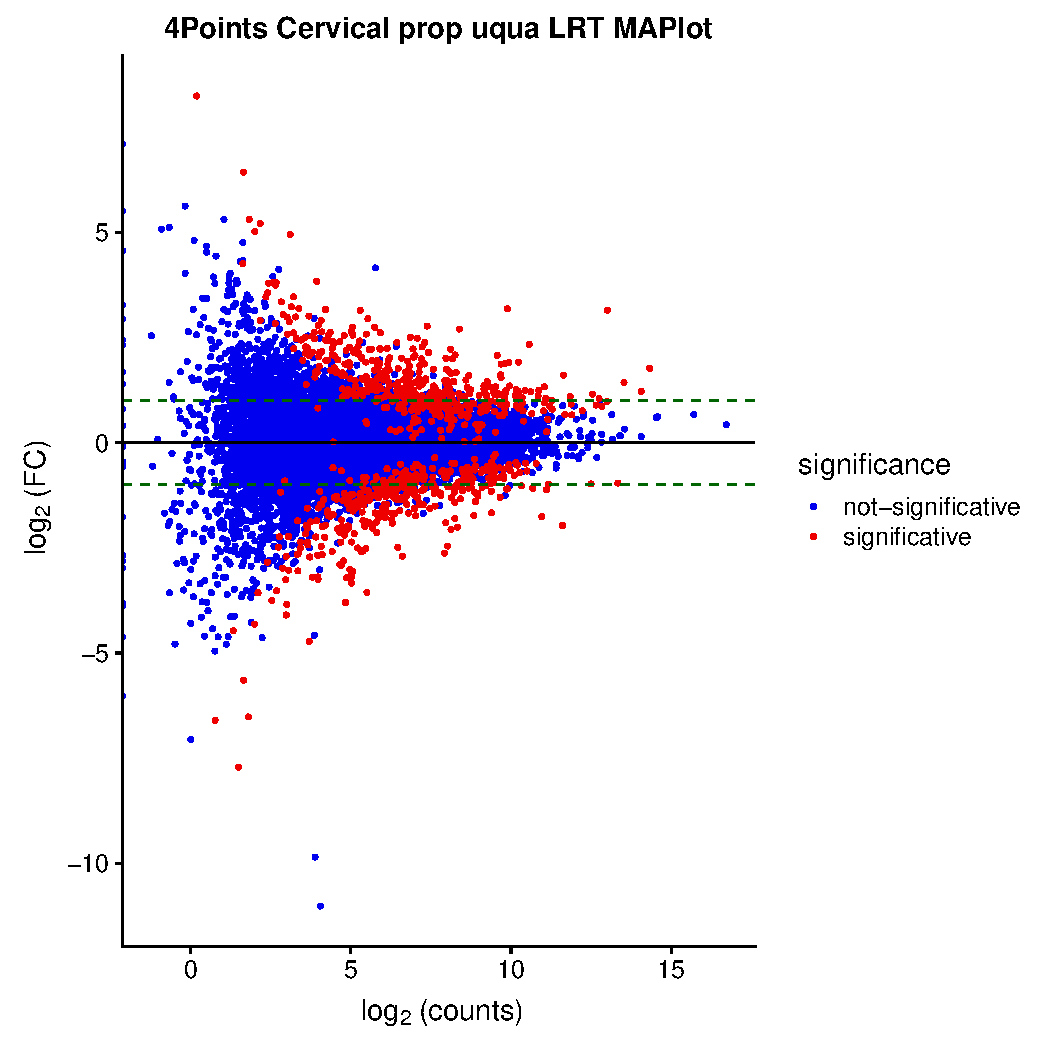
\includegraphics[width=\textwidth, keepaspectratio]{img/ticorser/de/volcma.pdf}
\caption[ticorser Volcano-MA plots]{An inspection of the results using a volcano plot (on the left) and an MA-Plot (on the right).}
\label{fig:ticorservolcma}
\centering
\end{figure}

In order to better compare the results coming from different analysis and methodologies approaches we can use one of the VENN diagrams available in \gls{tic}, which, while intersecting the results, saves all the gene lists coming from the intersections and also from exclusions.
Moreover, by setting the \lstinline!enrich.lists.flag! to \lstinline!TRUE!, the methods automatically start functional enrichment for both pathways (on \textit{Reactome} and \textit{KEGG} databases) and Gene Ontology (on \gls{gomf}, \gls{gocc} and \gls{gobp}), storing all the results in the \lstinline!output.folder! specified (we remind to next section for further details on Functional Enrichment Analysis).

\begin{figure}[H]
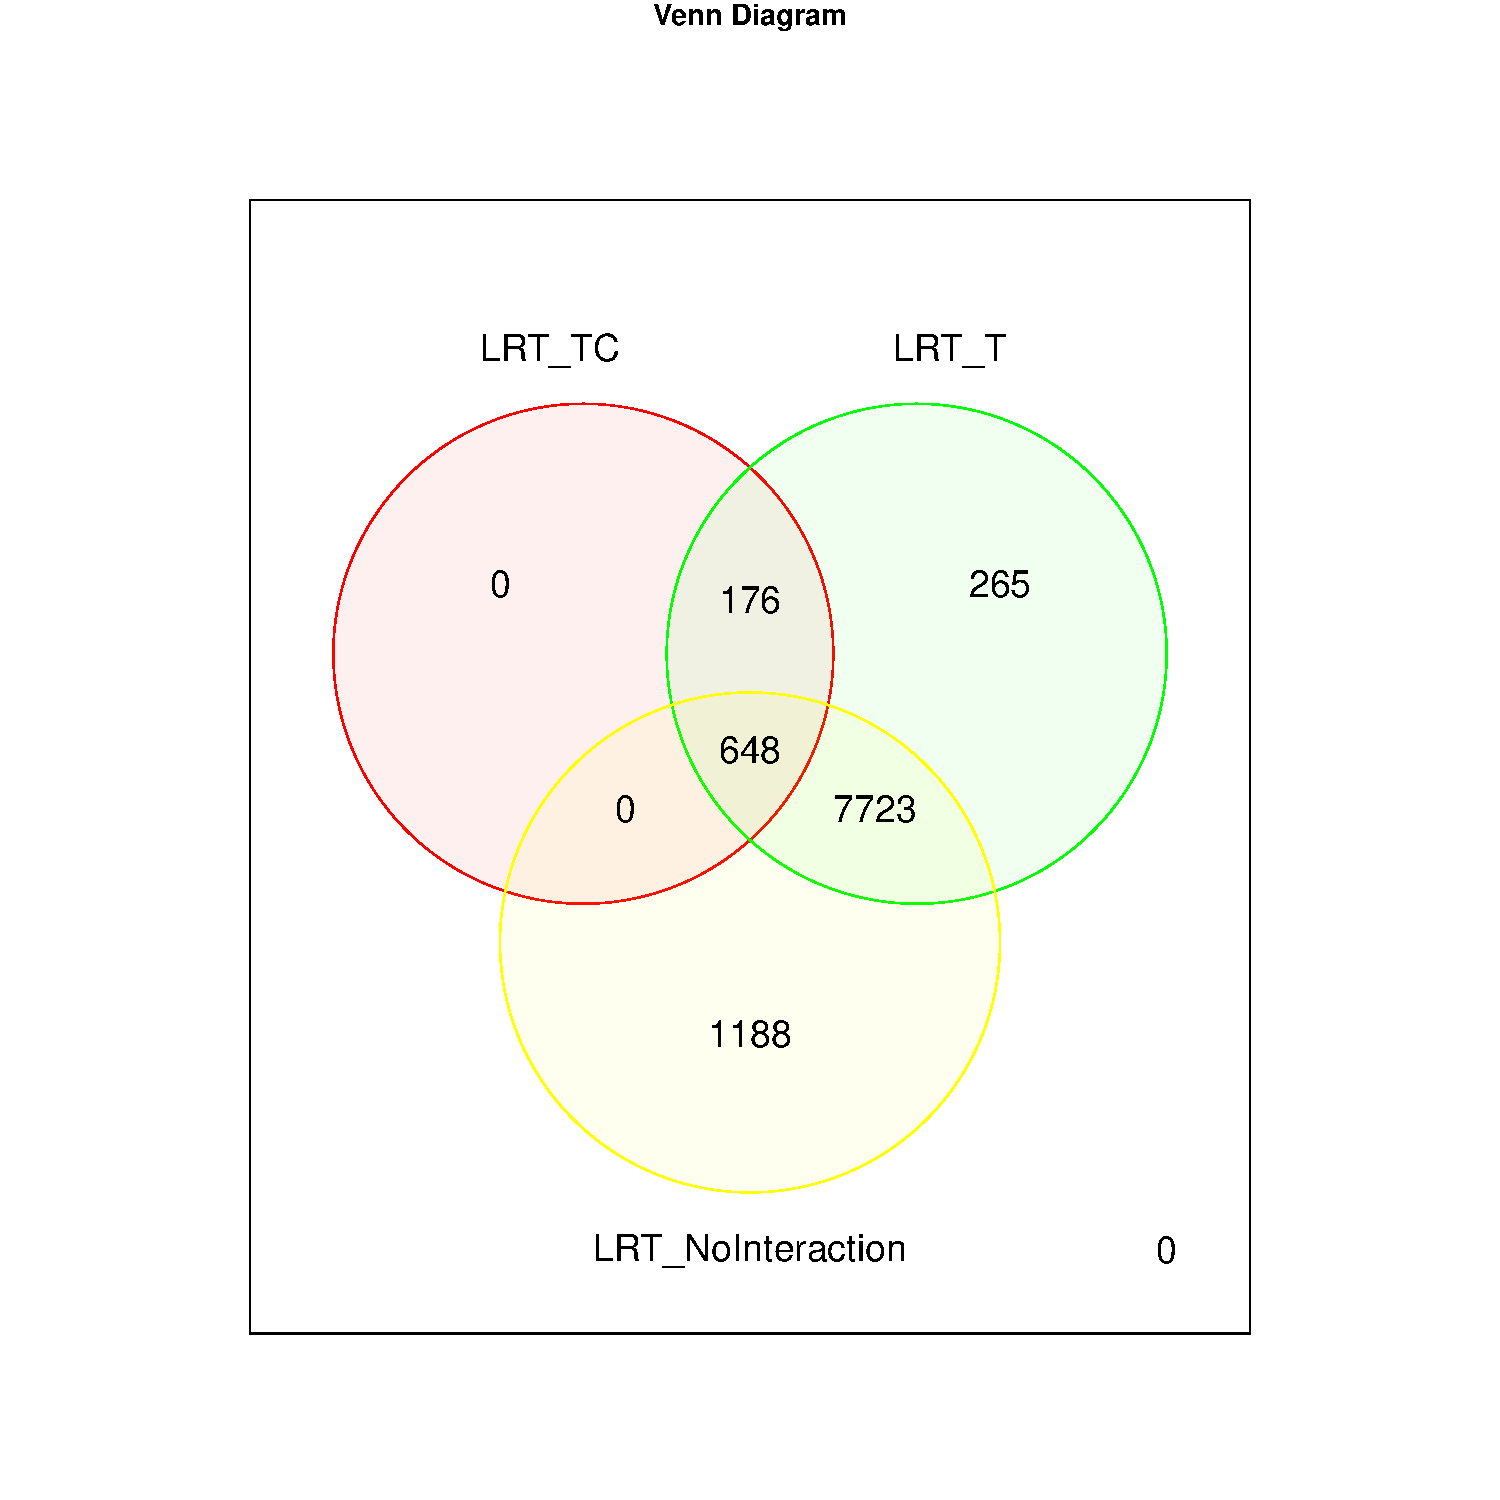
\includegraphics[width=\textwidth,height=\textheight,keepaspectratio]{img/ticorser/de/venn3.pdf}
\caption[ticorser venn diagram]{A VENN diagram to compare the \glspl{deg} detected by the three different \gls{tc} methods of \gls{tic}.}
\label{fig:ticorservenn}
\centering
\end{figure}

Depending on the biological question under investigation, it can be useful to identify the unique genes for each method used in the time course differential expression analysis, or the genes coming from their intersections.

To look at the gene expression, \gls{tic} has a specific function to explore the trend of a specific gene across the time points between the two conditions. 
By the usage of the \lstinline!PlotCountsAlongTimes! and by specifying the name of a gene that is present in the count matrix, we are able to explore its behaviour.

\begin{figure}[H]
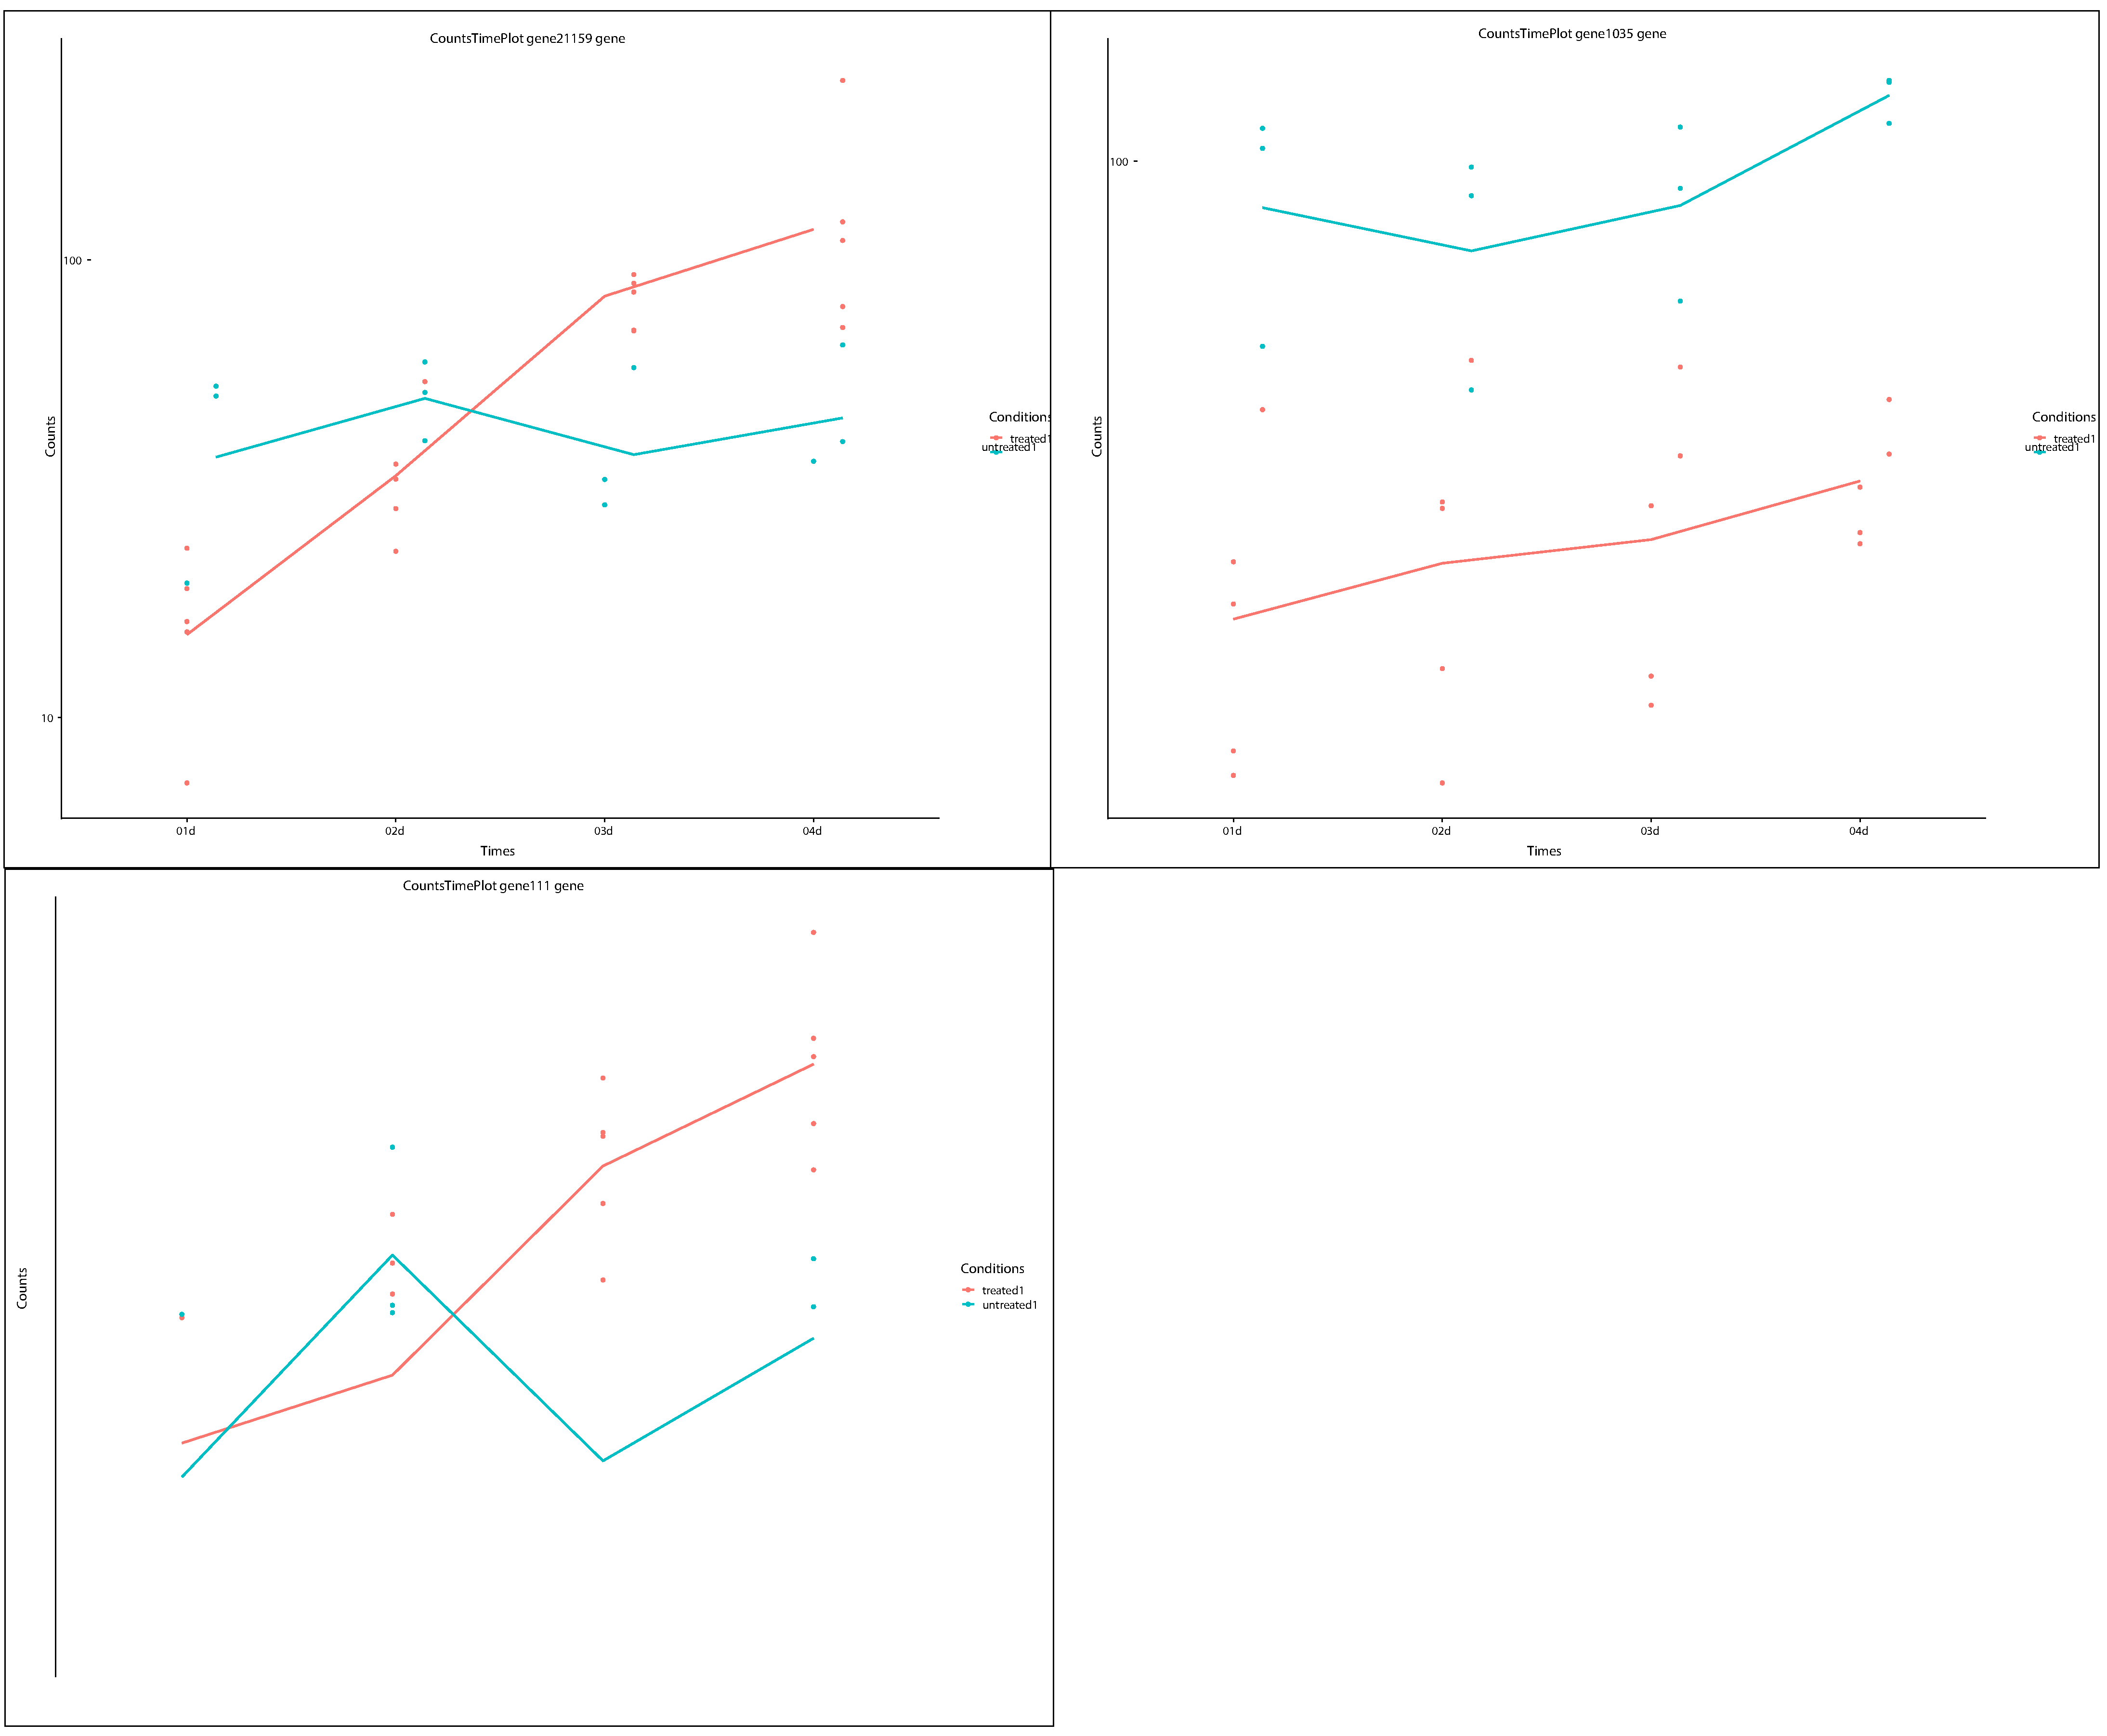
\includegraphics[width=\textwidth,keepaspectratio]{img/ticorser/de/trends/trends.pdf}
\caption[ticorser genes trends]{Three different trends examples of genes detected with \gls{tic} \textit{DE} \gls{tc} methods.}
\label{fig:ticorsertrends}
\centering
\end{figure}

For example looking at figure \ref{fig:ticorsertrends} we identified three different genes, one for each DE method, showing different trends over time points in conditions.
The first one is a gene detected by the \lstinline!DeSeqTime_TC! method, showing a complete inversion of the expression between the conditions during the time course experiment, otherwise, the second gene, detected with \lstinline!DeSeqTime_T! method, in the right upper corner, shows a difference between the conditions that remain unchanged across the experiment.
Finally, using the \lstinline!DeSeqTime_NoInteraction! method, we detected a gene with a \"strange\" behaviour, which is very oscillating across the time points and the conditions. 

Once inspected the results for the time course experiment analysis, an investigator could be interested in exploring the data on singular time points, here we report an analysis example on the first time point.

For the singular time point analysis, we can choose between four different methodologies, two present in the \textit{NOISeq} package (accessible through the \lstinline!ApplyNoiseq! function), the third one, the \textit{Wald test}, present in the \textit{DESeq2} package and, finally, the \textit{Quasi-likelihood} test from the \textit{edgeR} package.
It is a good practice to use more than one method while working with transcriptomic data in order to be more confident about the final results.
Table \ref{tab:ticorserderesultstp} illustrates differences between the methods used for \glspl{deg} detection.

For the motivations mentioned into the section \ref{sec:ticorseintromethods}, we use the \textit{NOISeqBio} method, and not the \textit{NOISeq} method, because we have biological replicates.


\begin{table}[H]
\centering
\begin{tabular}{r c c c}
%\cline{2-4}\cline{6-8}
%\cline{2-4}\cline{6-8}
\multicolumn{1}{r}{} & \multicolumn{3}{c}{Genes} \\
\cline{2-4}
\multicolumn{1}{r}{} & Total & UP & DOWN \\
\cline{2-4}
DESeq2 & 5239 & 2684 & 2555 \\
edgeR & 7095 & 2935 & 4170 \\
NOISeqBio & 6315 & 3053 & 3262 \\
\end{tabular}
\caption[\gls{tic} Single Time Points DE methods results]{A comparison of the number of \glspl{deg} detected with \gls{tic} at single time point. Here we present the results for the first time point (t01).}
\label{tab:ticorserderesultstp}
\end{table}

Figure \ref{fig:ticorsertpvenn} shows differences in the detection of \glspl{deg} using the three different methods.
In particular, \lstinline!NOISeqBio! is really useful when working with biological replicates (like in this case), indeed it is able to detect much more \glspl{deg} than the other methods. 
Indeed, when using \lstinline!NOISeq! on the same data, the \glspl{deg} are only 24, while \textit{DESeq2} is able to detect quite the same amount of genes.

\begin{figure}[H]
\centering
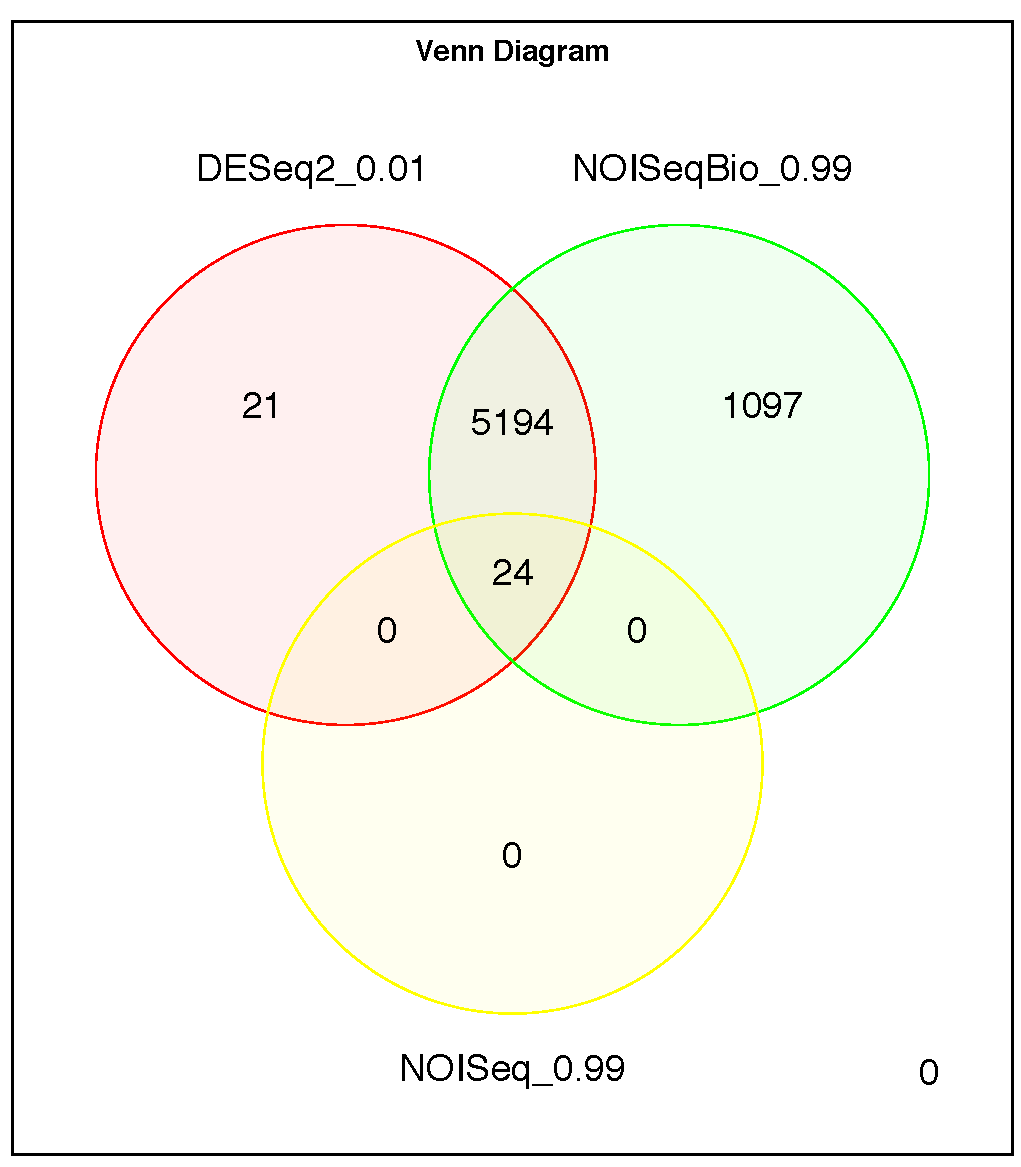
\includegraphics[width=10cm, keepaspectratio]{img/ticorser/de/singleTP/venn.pdf}
\caption[ticorser venn diagram single time point]{A venn diagram for comparying results coming from different methods used for \gls{deg} detection.}
\label{fig:ticorsertpvenn}
\end{figure}

It is also possible to use a singular function, \lstinline!PerformDEAnalysis!, for applying the preferred method in the differential expression phase. 
The tool automatically stores the results in the \lstinline!output.folder! creating an articulate, but intuitive, folder tree with all the results and the plots (Volcano and MA Plots), and performing functional enrichment analysis on the computed results, simply by setting the \lstinline!enrich.results.flag! to \lstinline!TRUE!.

\subsubsection{Functional Enrichment Analysis}

For the Functional Analysis \gls{tic} has a set of functions helping to perform it with \textit{GProfiler} and \textit{ClusterProfiler} tools \cite{Yu2012, Reimand2016}.

In order to perform pathway analysis with \textit{GProfiler} we used \lstinline!enrichPathwayGProfiler! function, twice, one for the \textit{Reactome} database and one for the \textit{KEGG} database enrichment.
Then, we performed the same analysis with \textit{ClusterProfiler} by using the \lstinline!enrichKEGGFunction!, which performs only on \textit{KEGG} database but is able to produce a graphical representation of the network of the pathways (see figure \ref{fig:ticorserpathmap}).

\begin{figure}[H]
\centering
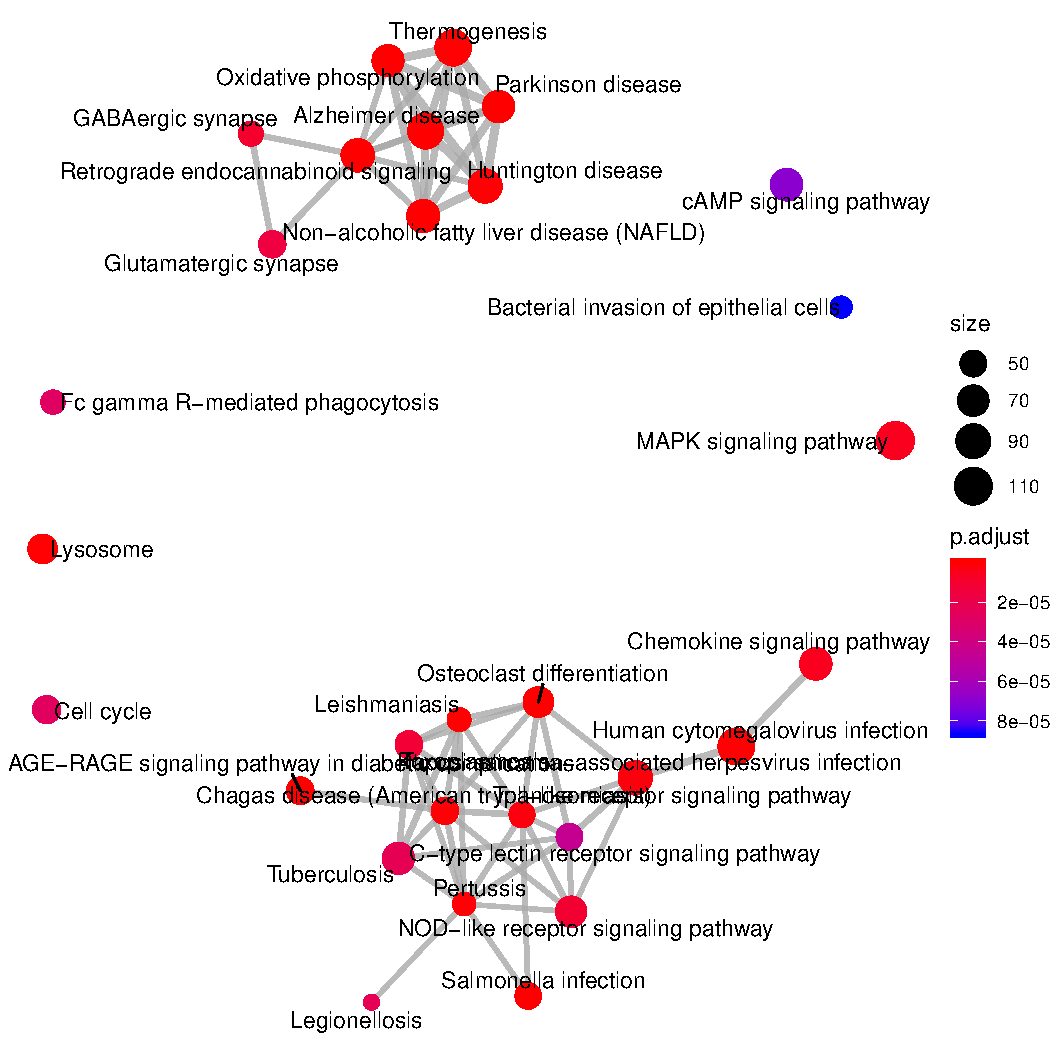
\includegraphics[width=\textwidth, keepaspectratio]{img/ticorser/functional/net_kegg.pdf}
\caption[ticorser pathway network]{A network representation of the \textit{KEGG} results obtained with \textit{clusterProfiler}package, by using \gls{tic}}
\label{fig:ticorserpathmap}
\end{figure}

On the other hand, to perform a \gls{go} functional enrichment analysis we use \lstinline!enrichGOGProfiler! three times, one for each class of the \lstinline!ontology!, \lstinline!CC! for Cellular Components, \lstinline!BP! for Biological Processes and \lstinline!MF! for Molecular Functions.
Analogously, we use \lstinline!enrichGOFunction! for performing the same analysis with \textit{ClusterProfiler}, which produces not only the table of the results but also a tree for the Gene Ontology terms significative in our dataset. (see figure \ref{fig:ticorsergo}).

Because the data used for this analysis have not been yet published, we do not publish the results obtained with \textit{clusterProfiler} and \textit{gProfiler}, but we show some relevant plots useful for illustrating the obtained results.

\begin{figure}[H]
\centering
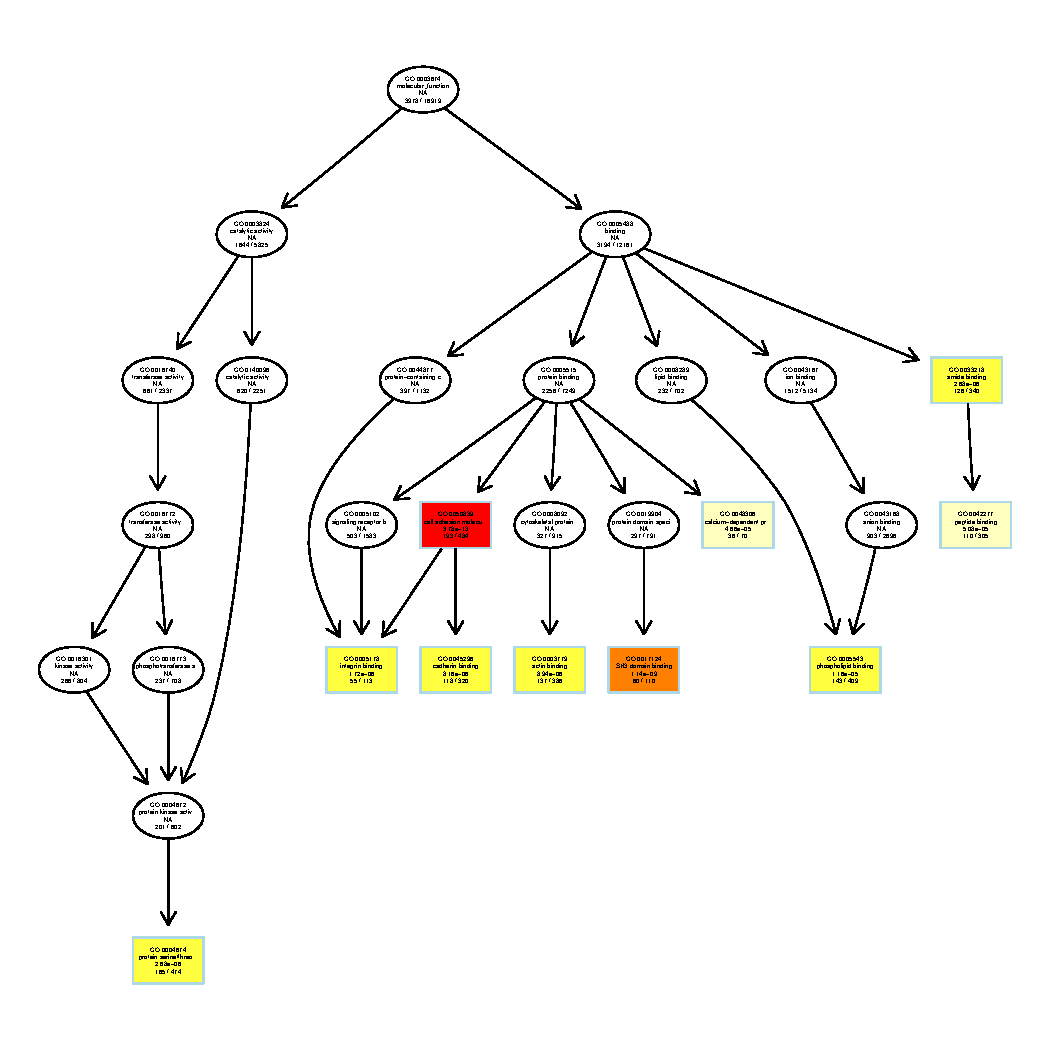
\includegraphics[width=\textwidth, keepaspectratio]{img/ticorser/functional/mf_hier.pdf}
\caption[ticorser hierarchial GO-terms]{A hierarchical graphical representation of Molecular Function GO-terms obtained with \textit{clusterProfiler}, by using \gls{tic}.
Graphical colours, from red (most significant) to yellow (less significant) indicates the p-value significance of each GO-term. 
Gray ones, are not significant at all.}
\label{fig:ticorsergo}
\end{figure}

Finally, when we identify one or more interesting \textit{KEGG} pathways, we can plot a \textit{KEGG map} representation of it, by using \lstinline!PlotKeggMapTimeCoursePathview!, which takes as input a data frame of relevant genes expression values for the interested pathway, and the \lstinline!keggid! identifying the pathway. 
In such a way a \textit{KEGG} map with the expression values at each time point for those genes will be visualized.
Figure \ref{fig:ticorserparkinson} and \ref{fig:ticorseralzheimer} graphically shows the \textit{KEGG-maps} of the \textit{Parkinson disease} and \textit{Alzheimer disease} pathways, which both resulted highly significant from our functional analysis, and which are known to be associated to \gls{sci} \cite{Yeh2016, Yeh2018}.

\begin{figure}[H]
\centering
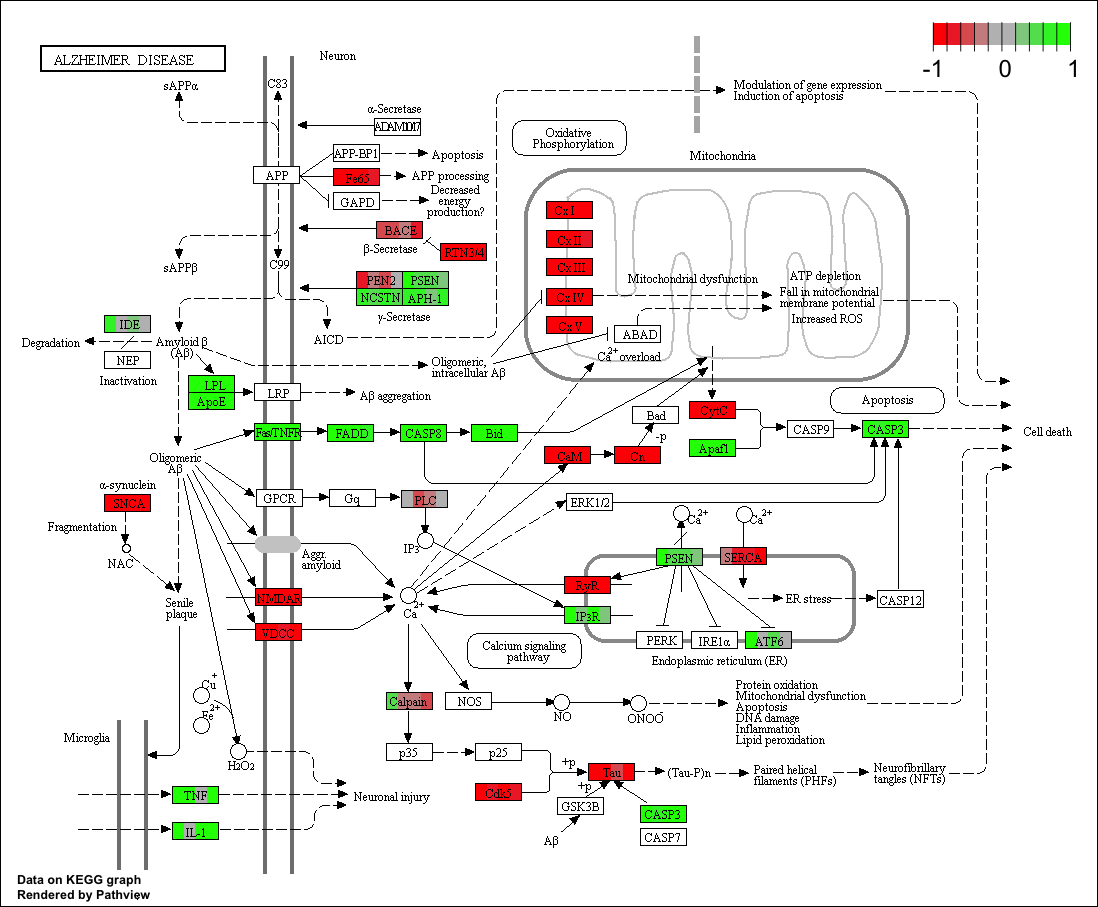
\includegraphics[width=\textwidth, keepaspectratio]{img/ticorser/functional/alzheimer.png}
\caption[ticorser alzheimer keggmap]{A keggmap for Alzheimer disease. Each \gls{deg} is coloured depending on the log2(fc) of its expression. Moreover, for each highlighted gene, the box is divided in 4 "mini-boxes", one for each time point.}
\label{fig:ticorseralzheimer}
\end{figure}

\begin{figure}[H]
\centering
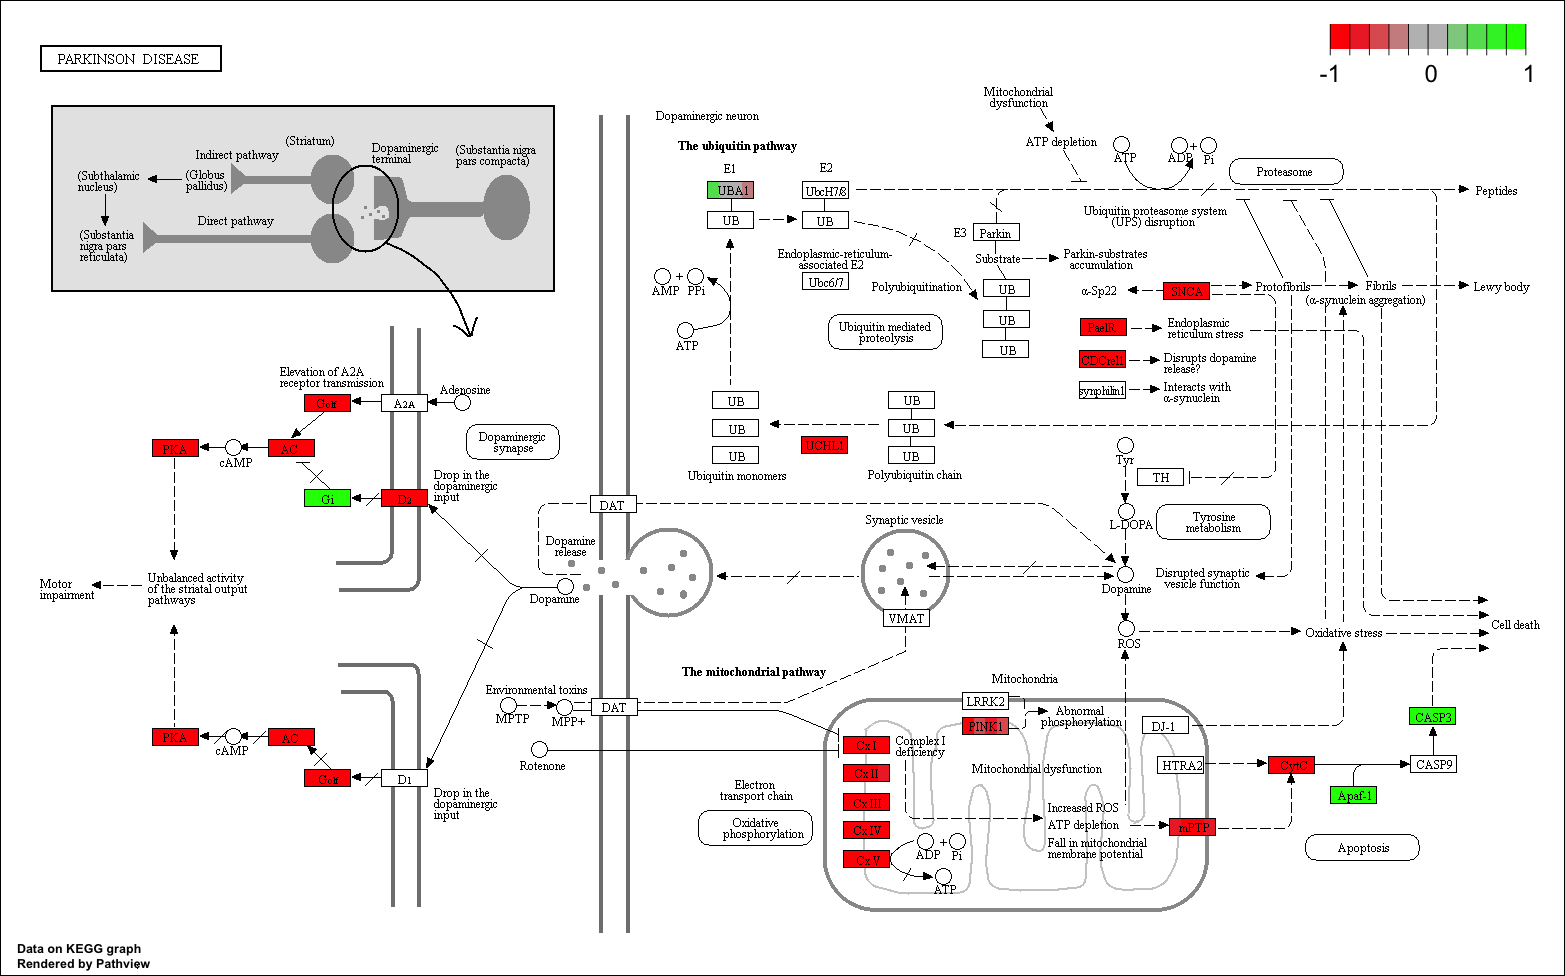
\includegraphics[width=\textwidth, keepaspectratio]{img/ticorser/functional/parkinson.png}
\caption[ticorser parkinson keggmap]{A keggmap for Parkinson disease. Each \gls{deg} is coloured depending on the log2(fc) of its expression. Moreover, for each highlighted gene, the box is divided in 4 "mini-boxes", one for each time point.}
\label{fig:ticorserparkinson}
\end{figure}






